
% Single column for now
%\documentclass[conference]{IEEEtran}
\documentclass{article}

\usepackage{graphicx}
\graphicspath{{figures/}}
\DeclareGraphicsExtensions{.pdf,.jpeg,.png,.eps}
\usepackage[cmex10]{amsmath}
\usepackage{amsfonts}
\usepackage{amssymb}
\usepackage{algorithmic}
\usepackage{array}
\usepackage{mdwmath}
\usepackage{mdwtab}
\usepackage{eqparbox}
\usepackage[tight,footnotesize]{subfigure}
\usepackage[caption=false,font=footnotesize]{subfig}
\usepackage{fixltx2e}
\usepackage{stfloats}
\usepackage{url}

% correct bad hyphenation here
% Math definitions
\newcommand{\norm}[1]{\left\Vert#1\right\Vert}
\newcommand{\abs}[1]{\left\vert#1\right\vert}
\newcommand{\set}[1]{\left\{#1\right\}}
\newcommand{\To}{\longrightarrow}
\newcommand{\Ker}{\textup{Ker}}
\newcommand{\Img}{\textup{Img}}
\newcommand{\diag}{\textup{diag}}
\newcommand{\circulant}{\textup{circ}}
\newcommand{\bcf}{\;\mbox{\boldmath ${\cal F}$\unboldmath}}
\def\Vec#1{\!\!\hbox{$#1$\kern-0.38em\lower0.85em\hbox{$\vec{}\,$}}\,}%
\newcommand{\bbm}{\begin{bmatrix}}
\newcommand{\ebm}{\end{bmatrix}}
\newcommand{\mbf}[1]{\mathbf{#1}}
\newcommand{\mbs}[1]{{\boldsymbol{#1}}}
\newcommand{\mbb}[1]{{\mathbb{#1}}}
\newcommand{\mc}[1]{\mathcal{#1}}
\newcommand{\argmin}{\operatornamewithlimits{argmin}}
\newcommand{\argmax}{\operatornamewithlimits{argmax}}
\newcommand{\expect}{\operatornamewithlimits{\mbb{E}}}

\begin{document}

\title{Sparse Planning Graphs for Information Driven Simultaneous Localization and Mapping}

% This block only works in IEEE mode
%\author{\IEEEauthorblockN{1,2,3}
%  \IEEEauthorblockA{The Robotics Institute\\
%    Carnegie Mellon University\\
%    Pittsburgh, PA 15217\\
%Email: \{1,2,3\}@cmu.edu}}

\maketitle

\begin{abstract}
  \boldmath
  \dots
\end{abstract}

\section{Introduction}
\label{sec:introduction}

% Motivation
Exploration is a key capability that enables robotic vehicles to operate in
unknown environments. In this project we develop an active perception policy
for robotic exploration. Active perception exploration formulations
choose control actions which optimize an information-theoretic objective
function such as Shannon's mutual information or entropy
\cite{bourgault2002information, stachniss2005information} over the robot's map,
given a sensor measurement model. Other common exploration techniques, such as frontier
exploration \cite{}, use geometric reasoning to infer explorative paths.
While these strategies work well in practice, they operate on a
maximum likelihood estimate of the map, and apply heuristics to determine the most uncertain
locations in the environment. In contrast, active perception strategies do not utilize
geometric or maximum likelihood assumptions, and instead interpret the map as a binary
random variable, choosing actions which directly minimize the random variable's uncertainty.
Additionally, information-based exploration methods easily extend to 3D
configuration spaces, a benefit which is not shared by frontier methods.
Julian et al. prove that maximizing mutual information between a
robot's map and expected future map naturally yields explorative behaviors
\cite{julian2013mutual}.

% Overview of our approach
Active perception formulations seek to optimize information-theoretic
objectives. While this optimization is real-time for short planning horizons,
these metrics are often expensive to compute online, requiring double
integration over possible future robot states and measurements, or Monte Carlo sampling
from the distribution of measurements. These expensive per-pose computations inhibit
online dense evaluation over a configuration space. In this project, we aim to develop an
efficient active perception exploration strategy which evaluates the
information-theoretic objective in a sparse, but well-chosen set of poses across the
configuration space. This strategy evaluation the objective function
a limited number of times, while still generating paths that sufficiently explore the space.

% Overview of RRT
To achieve real-time active perception exploration, we use a Rapidly-Exploring Random Tree
(RRT) to generate sets of dynamically feasible actions over a finite planning horizon
\cite{Kuwata09_TCST}. RRT planners trade trajectory optimality for efficiency, allowing for evaluation
of many potential future locations in the configuration space during a single planning
step. In addition, RRT planners are anytime, and generate potential trajectories
for a pre-specified amount of time before evaluating the most optimal sampled trajectory. Our
strategy evaluates each RRT leaf-node using the information-theoretic objective function,
and stores the resulting reward in the tree. After planning for a specified
amount of time, the maximum reward leaf-node is chosen as the optimal location to
visit, and the RRT is traversed to generate a dynamically feasible trajectory to
that location.

% Overview of CSQMI
In addition to the efficiency gains from using an RRT, a recent work by Charrow
et al. \cite{charrow15} has
proposed the Cauchy-Schwarz Quadratic Mutual Information (CSQMI) as an efficient
information-theoretic objective function. CSQMI is theoretically
well-motivated: it is derived from Renyi's Quadratic Entropy, a generalization of Shannon's entropy.
However, in contrast to Shannon's mutual information (which is derived directly
from Shannon's entropy), CSQMI is shown to have superior computational efficiency.

% Results and implementation
The contribution of this work is an exploration framework to enable online exploration using CSQMI in sparse
planning graphs, such as RRTs. We demonstrate an implementation of our approach
in simulation, and provide analysis of experiments in which a mobile ground
robot must explore an unknown space using a laser scanner range sensor. We discuss the
formulation and implementation of the CSQMI metric, RRT, and a controller and
Unscented Kalman Filter (UKF) that were developed to enable trajectory tracking and
state estimation. Finally, we discuss the implementation of these capabilities
on a real ground robot.

% Overview of sections
This paper is structured in the following manner: Section~\ref{sec:occupancy_grid_mapping}
gives a brief overview of occupancy grid mapping which is necessary for the CSQMI
information metric. Section~\ref{sec:information_theoretic_objective}
details the CSQMI information-theoretic cost objective and its similarities to
Shannon's mutual information. Section~\ref{sec:measurement_model} discusses the
measurement model that was chosen to evaluate expected future measurements.
Sections~\ref{sec:planner} and~\ref{sec:unscented_kalman_filter} cover the RRT and UKF formulations
used in our implementation. Finally, Sections~\ref{sec:results}
and~\ref{sec:conclusion} give results and analysis of our implementation in
simulation, and describe future work towards implementing our algorithms on a
ground robot.


\section{Exploration Cost Functional}
\label{section:exploration_cost_functional}

The purpose of the planner is to find a dynamically feasible series of control actions from a set of motion primitives, $\mc{X}$, over a time interval, $\tau := t+1 : t+T$, which enable the robot to gather observations that maximize an information metric over its map. We define an \textit{action} as a discrete sequence of states, $x_{\tau} = \left[x_{t+1},\dots,x_{t+T}\right]$. While executing an action, the robot will obtain a set of measurements $z_{\tau}(x_{\tau}) = \left[z_{t+1},\dots,z_{t+T}\right]$ by sensing from the states $x_{\tau}$. Under this notation, the planner must determine $x_{\tau}^{*}$, the action that visits locations which allow the robot to obtain the set of measurements, $z_{\tau}^{*}$, which, when integrated into the map, maximize an information-theoretic cost function over the map. We choose to maximize Shannon Mutual Information rate between the current map, $m$, and the measurements $z_{\tau}$ gathered along $x_{\tau}$.
%
\begin{align}
  \begin{split}
    x_{\tau}^{*}
    &=
    \argmax_{x_{\tau} \in \mc{X}^{T}}
    \frac{\text{I}_{\text{MI}}
      \left[
        m
        ;
        z_{\tau}
        \ \vert \
        x_{\tau}
      \right]
    }
    {R\left(T\right)}
  \end{split}
\end{align}
%
where $\text{I}_{\text{MI}}$ is the Shannon Mutual Information.
%
\begin{align}
  \begin{split}
    \text{I}_{\text{MI}}
    \left[
      m
      ;
      z_{\tau}
    \right]
    &=
    \text{H}
    \left[
      m
    \right]
    -
    \text{H}
    \left[
      m
      \ \vert \
      z_{\tau}
    \right]
  \end{split}
\end{align}
%
Since the optimization is performed over $x_{\tau}$, the map entropy term can be removed.
%
\begin{align}
  \begin{split}
    x_{\tau}^{*}
    &=
    \argmax_{x_{\tau} \in \mc{X}^{T}}
    \frac{
      -
      \text{H}
      \left[
        m
        \ \vert \
        z_{\tau}
      \right]
    }
    {
      R
      \left(
      T
      \right)
    }
  \end{split}
\end{align}
%
Here we can make several assumptions to simplify the optimization of $x_{\tau}^{*}$. Due to cell independence in the occupancy grid formulation, the joint entropy over the map can be expressed as a sum of individual cell entropies. Additionally, let $\mc{C}$ to be the set of cells in the map that beams in $z_{\tau}$ pass through. We note that cells $c \notin \mc{C}$ are not updated by $z_{\tau}$ and therefore do not contribute to the map's conditional entropy. Using these assumptions, as well as the notation $p_c^{\tau} \equiv p(c \ \vert \ z_{\tau})$ and $o(c \ \vert \ z_{\tau}) \equiv p_{c}^{\tau}\log p_{c}^{\tau} + (1 - p_{c}^{\tau})\log (1 - p_{c}^{\tau})$, we may write the entropy of the map conditioned on $z_{\tau}$ as
%
\begin{align}
  \begin{split}
    \text{H}
    \left[
      m
      \ \vert \
      z_{\tau}
    \right]
    &=
    \sum_{c \in \mc{C}}
    \text{H}
    \left[
      c
      \ \vert \
      z_{\tau}
    \right]
    \\
    &=
    \sum_{c \in \mc{C}}
    \expect_{c, z_{\tau}}
    \left[
      -\log
      p
      \left(
      c
      \ \vert \
      z_{\tau}
      \right)
    \right]
    \\
    &=
    -
    \int_{z_{\tau}}
    p
    \left(
    z_{\tau}
    \right)
    \sum_{c \in \mc{C}}
    o
    \left(
    c
    \ \vert \
    z_{\tau}
    \right)
    d z_{\tau}
    \label{eq:conditional_entropy}
  \end{split}
\end{align}
%
Integration over the space of measurements $z_{\tau}$ is computationally intractable. Instead, we approximate Eq.~\eqref{eq:conditional_entropy} using $N$ Monte Carlo samples from the distribution $p(z_{\tau})$.
%
\begin{align}
  \begin{split}
    \text{H}
    \left[
      m
      \ \vert \
      z_{\tau}
    \right]
    &\approx
    -\frac{1}{N}
    \sum_{i=1}^{N}
    \sum_{c \in \mc{C}}
    o
    \left(
    c
    \ \vert \
    z_{\tau}^{i}
    \right)
    \\
  \end{split}
\end{align}
%
\begin{align}
  \begin{split}
    x_{\tau}^{*}
    &=
    \argmax_{x_{\tau} \in \mc{X}^{T}}
    \frac{1}{R\left(T\right)}
    \sum_{i=1}^{N}
    \sum_{c \in \mc{C}}
    o
    \left(
    c \ \vert \ z_{\tau}^{i}
    \right)
  \end{split}
\end{align}
%
\subsection{Measurement Model}

As explained in Sect.~\ref{section:exploration_cost_functional}, each future position $x_{k}$ will generate a multi-beam range measurement $z_{m}$. We express each measurement as a $K$-tuple random variable, $z_{m} = \left[z_{m}^{1}, \dots, z_{m}^{K}\right]$, with $z_{m}^{k} \in \left[z_{min}, z_{max}\right]$. A measurement model is required to sample from the distribution $p(z_{\tau} \ \vert \ m)$. Assuming laser beam independence, $p(z_{\tau} \ \vert \ m)$ can be expressed as a product of the measurement probabilities of individual beams at each timestep over the interval $\tau = t+1:t+T$.
%
\begin{align}
  \begin{split}
    p
    \left(
    z_{\tau}
    \ \vert \
    m
    \right)
    &=
    \prod_{m=t+1}^{t+T}
    \prod_{k=1}^{K}
    p
    \left(
    z_{m}^{k}
    \ \vert \
    m
    \right)
  \end{split}
\end{align}
%
The probability of a single beam measurement can be expressed as a function of the true distance, $r$, to the obstacle.
%
\begin{align}
  \begin{split}
    p
    \left(
    z_{m}^{k}
    \ \vert \
    m
    \right)
    &=
    \int_{r}
    p
    \left(
    z_{m}^{k}
    \ \vert \
    r
    ,
    m
    \right)
    p
    \left(
    r
    \ \vert \
    m
    \right)
    dr
  \end{split}
\end{align}
%
\begin{align}
  \begin{split}
    p
    \left(
    z_{m}^{k}
    \ \vert \
    r
    ,
    m
    \right)
    &=
    \left\{
    \begin{array}{ll}
      \mc{N}(z_{m}^{k} - r, \sigma_{hit}^{2}) &: z_{min} \le r \le z_{max} \\
            \mc{N}(z_{max}, \sigma_{hit}^{2}) &: z_{max} < r \\
                                            0 &: r < z_{min}
    \end{array}
    \right.
    \label{eq:measurement_model}
  \end{split}
\end{align}
%
where $\mc{N}(x - \mu, \sigma^{2})$ is a one-dimensional Gaussian with mean $\mu$ and variance $\sigma^{2}$. The Gaussian term in Eq.~\eqref{eq:measurement_model} is an approximation for the true distribution, which is a complex function of both beam angle as well as non-axial distance-dependent noise. The environment-dependent distribution $p(r)$ corresponds to the probability that an obstacle intersects a beam at range $r$. We model this as a Poisson binomial distribution with probabilities decaying according to the inverse square of the beam range.

On the interval $\left[z_{min}, z_{\max}\right]$, $p(z_{m}^{k})$ reduces to a Gaussian convolution with $p(r)$ over $r$, which can be computed in $O(n \log n)$ operations with a Fast Fourier Transform. This computation can be reduced to $O(n)$ by assuming that $\sigma_{hit}$ of the range sensor is much smaller than the resolution of the map.

The distribution $p(r)$ represents the probability that the first obstacle along a ray originating at the sensor is found at distance $r$. $p(r)$ can be expressed as a generalization of the geometric distribution for independent, but not identically distributed (i.n.i.d.) Bernoulli trials.
%
\begin{align}
  \begin{split}
    p(r = i
    \ \vert \
    m)
    &=
    p_{t}(m^i)
    \prod_{j=1}^{i-1}
    \left(
      1 - p_{t}(m^{j})
    \right)
    \\
    &=
    p_{t}(m^i)
    \left(
      \frac{1}{p_{t}(m^{i-1})} - 1
    \right)
    p(r = i - 1
    \ \vert \
    m)
  \end{split}
\end{align}


\begin{figure}
  \centering
  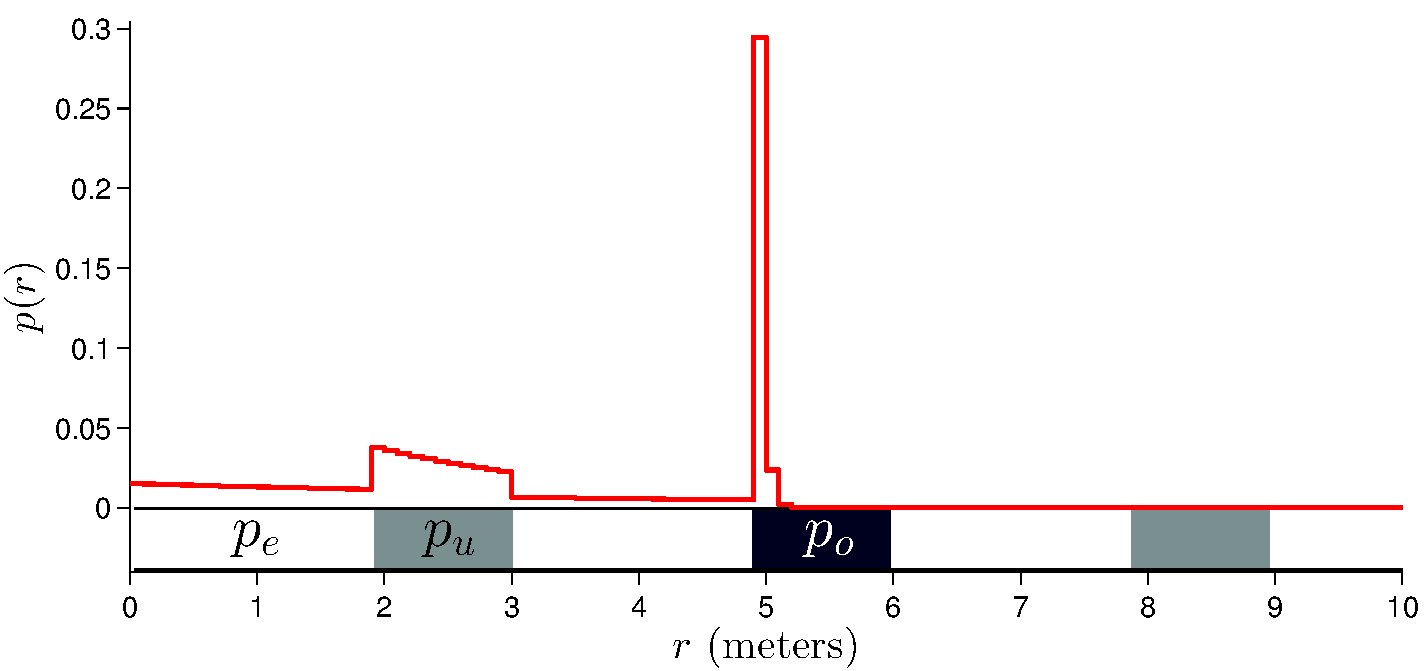
\includegraphics[width=0.5\textwidth]{meas_model.pdf}
  \caption{The distribution $p(r \ \vert \ m)$ over a depicted 1-dimensional map with resolution $\Delta r = 0.1$ m, and $p_{e} = 0.01$, $p_{o} = 0.92$, $p_{u} = 0.05$. \label{fig:measurement_model}}
\end{figure}





































\iffalse
Our goal is to enable receding horizon planning for active SLAM in a computationally tractable formulation. The active SLAM exploration problem can be framed as determining the control actions which guide a robot to a state that maximizes mutual information between its current and future maps. Efficient implementations of active SLAM allow robots to plan several control actions into the future. In this section we detail a sparse graph-based architecture which enables efficient updates to estimated mutual information gains at future poses upon acquiring new observations. This solution allows us to plan many steps into the future, with guarantees on the maximum horizon distance at which it is no longer feasible to compute an optimal plan in real-time.

We model the map as an occupancy grid, and represent the map as a conglomeration of cells: $m = \{m^{i}\}_{i=1}^{N}$. The probability that an individual cell is occupied at $t$ is given by $p\left(m^{i} \ \vert \ x_{1:t}, z_{1:t}\right)$, where $x_{1:t}$ denotes the history of states of the vehicle, and $z_{1:t}$ denotes the history of range observations accumulated by the vehicle. Additionally we assume that cell occupancies  are independent of one another: $p\left(m \ \vert \ x_{1:t}, z_{1:t}\right) = \prod_{i} p\left(m^{i} \ \vert \ x_{1:t}, z_{1:t}\right)$. For notational simplicity we write the map conditioned on random variables $x_{1:t}$ and $z_{1:t}$ as $p\left(m_{t}\right) := p\left(m \ \vert \ x_{1:t}, z_{1:t}\right)$.

The optimal plan over a one step horizon will guide the robot to a state, $x_{t+1}^{*}$, in which the mutual information between $m_{t}$ and $m_{t+1}$ is maximized.

\begin{align} \begin{split}
  x_{t+1}^{*}
  &=
  \argmax_{x_{t+1}}
  \
  \text{IG}\left[
    m_{t}
    ;
    m_{t+1}
  \right]
  \\
  &=
  \argmax_{x_{t+1}}
  \
  \text{H}\left[
    m_{t}
  \right]
  -
  \expect_{z_{t+1}}\left[
    \text{H}\left[
      m_{t+1}
    \right]
  \right]
  \\
  &=
  \argmin_{x_{t+1}}
  \
  \expect_{z_{t+1}}\left[
    \text{H}\left[
      m_{t+1}
    \right]
  \right]
\end{split} \end{align}

The term $\text{H}\left[m_{t}\right]$ is independent of the future state $x_{t+1}$, so the information gain is maximized when $x_{t+1}$ minimizes the expected entropy of the updated map. The independence between cell occupancies allows us to write the future entropy of the map as a sum of future entropies of individual grid cells:

\begin{align} \begin{split}
  \text{H}\left[
    m_{t+1}
  \right]
  &=
  \sum_{i=1}^{N}
  \text{H}\left[
    m_{t+1}^{i}
    \ \vert \
    m_{t+1}^{i-1}
    , \
    \dots
    \ ,
    m_{t+1}^{1}
  \right]
  \\
  &=
  \sum_{i=1}^{N}
  \text{H}\left[
    m_{t+1}^{i}
  \right]
  \\
  &=
  -\sum_{i=1}^{N}
  p\left(m_{t+1}^{i}\right)
  \log p\left(m_{t+1}^{i}\right)
  \\
  &\quad
  -\sum_{i=1}^{N}
  \left( 1 - p\left(m_{t+1}^{i}\right) \right)
  \log \left( 1 - p\left(m_{t+1}^{i}\right) \right)
\end{split} \end{align}

The expectation to minimize is therefore

\begin{align} \begin{split}
  \expect_{z_{t+1}}\left[
    \text{H}\left[
      m_{t+1}
    \right]
  \right]
  &=
  \int
  p\left(
  z_{t+1}
  \right)
  \sum_{i=1}^{N}
  \text{H}\left[
    m_{t+1}^{i}
  \right]
  dz_{t+1}
  \\
  &=
  -\expect_{z_{t+1}}\left[
    \sum_{i=1}^{N}
    \log p\left(
    m_{t+1}^{i}
    \right)
  \right]
\end{split} \end{align}

\section{Planner}
The purpose of the planner is to find a dynamically feasible series of control actions over a time interval, $\tau := t+1 : t+T$, through a metric space, $\mathcal{X}$, which enable the robot to gather observations that maximize an information metric over its map. We define an \textit{action} as a discrete sequence of states, $x_{\tau} = \left[x_{t+1},\dots,x_{t+T}\right]$. While executing an action, the robot will obtain a set of measurements $z_{\tau} = \left[z_{t+1},\dots,z_{t+T}\right]$ by sensing from the states $x_{\tau}$. Under this notation, the planner must determine $x_{\tau}^{*}$, the action that visits locations which allow the robot to obtain the set of measurements, $z_{\tau}^{*}$, which, when integrated into the map, maximize an information-theoretic cost function over the map. We choose to maximize Shannon Mutual Information rate between the current map, $m$, and the measurements $z_{\tau}$ gathered along $x_{\tau}$.

\begin{align} \begin{split}
  z_{\tau}^{*}
  &=
  \argmax_{z_{\tau}}
  \frac{\text{I}_{\text{MI}}\left[m_{t}; m_{\tau}\left(z_{\tau}\right) \right]}
  {T}
\end{split} \end{align}

The choice of mutual information rate, as opposed to mutual information, allows the planner to consider actions which differ in duration.

In typical 2D and 3D mobile robot planning problems, $\mathcal{X} = \mathcal{C}$, the configuration space, which contains a fixed obstacle region, $X_{obs} \subset \mathcal{X}$, and a complementary free space region, $X_{free} = \mathcal{X} \setminus X_{obs}$.
\fi



\end{document}








%\subsection{Subsection Heading Here}
%
%\begin{figure}[!t]
%\centering
%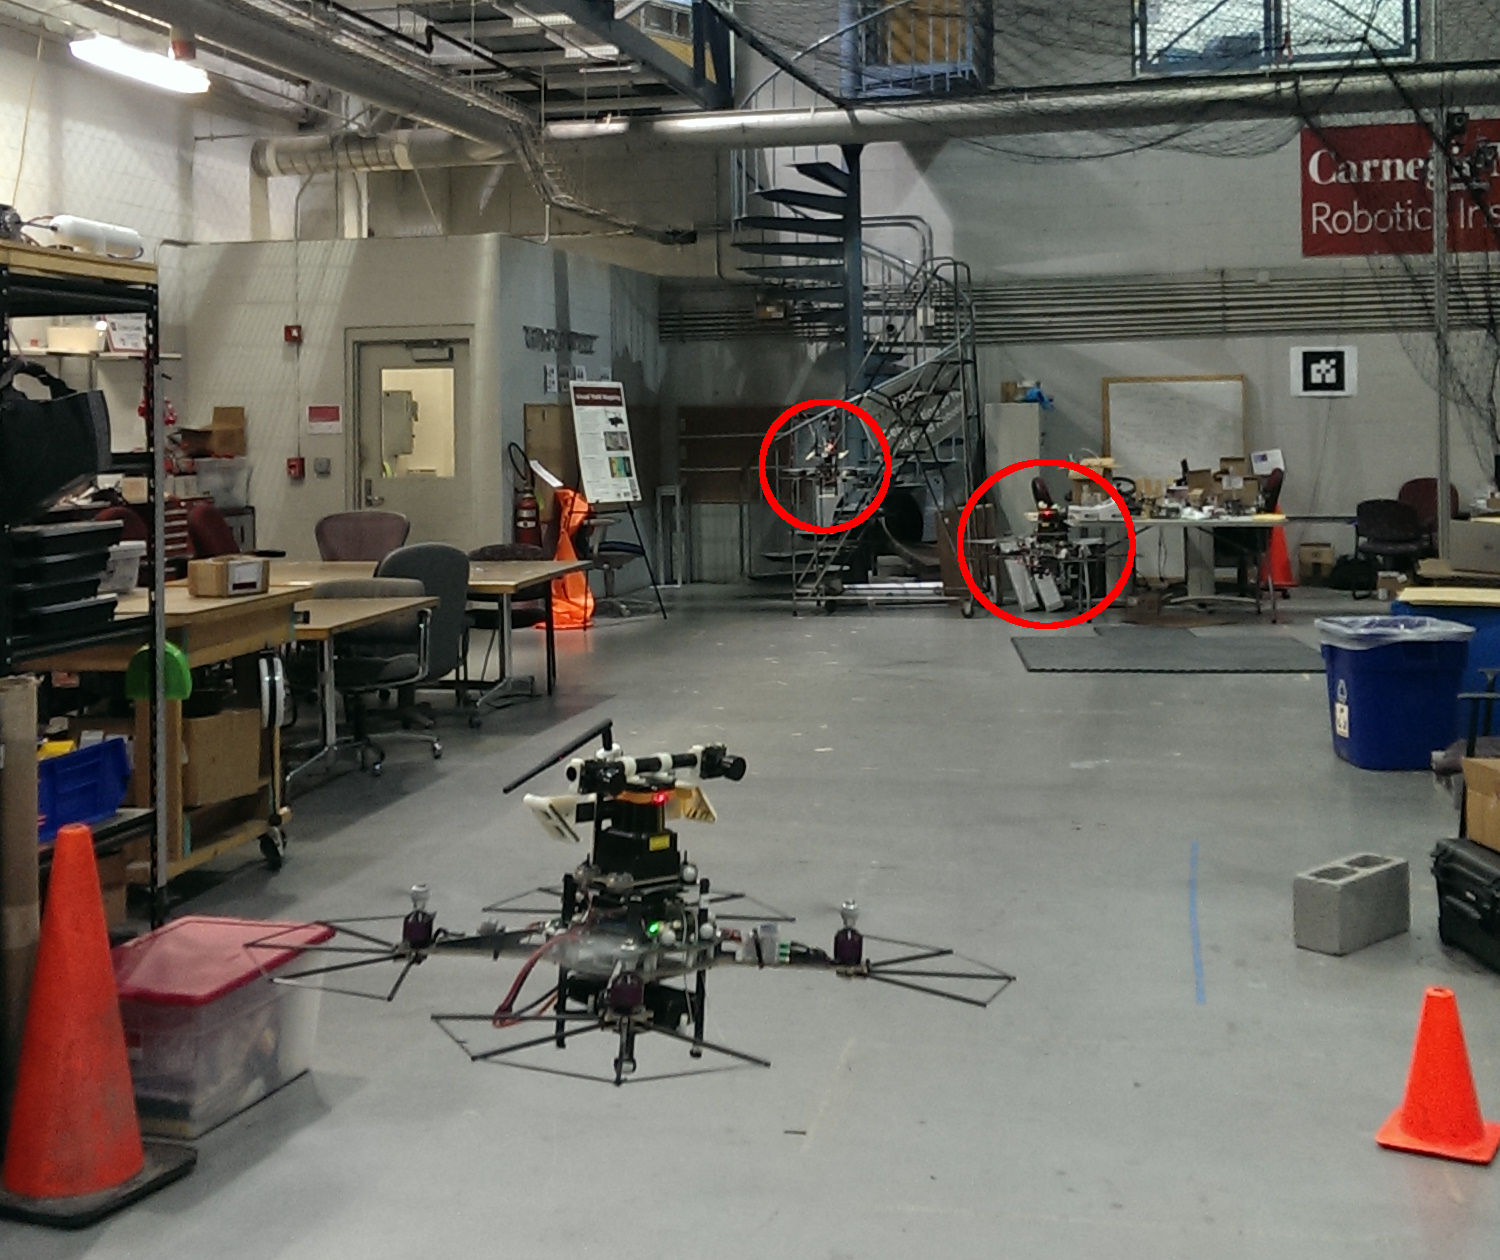
\includegraphics[width=2.5in]{3quads.png}
%\caption{Simulation Results}
%\label{fig_sim}
%\end{figure}
%\begin{table}[!t]
%\renewcommand{\arraystretch}{1.3}
%\caption{An Example of a Table}
%\label{table_example}
%\centering
%\begin{tabular}{|c||c|}
%\hline
%One & Two\\
%\hline
%Three & Four\\
%\hline
%\end{tabular}
%\end{table}

%\appendices
%\section{Proof of the First Zonklar Equation}

%\begin{thebibliography}{1}

%\bibitem{IEEEhowto:kopka}
%H.~Kopka and P.~W. Daly, \emph{A Guide to \LaTeX}, 3rd~ed.\hskip 1em plus
%  0.5em minus 0.4em\relax Harlow, England: Addison-Wesley, 1999.
%\end{thebibliography}
